%\documentclass[twocolumn]{elsart}
\documentclass{elsart}
\usepackage{amsmath,amssymb,graphicx,amsfonts, caption, subcaption, placeins}
\usepackage[english]{babel}
\usepackage{wrapfig}
\begin{document}
	%\textwidth 15cm \topmargin -1cm
	%\parindent 5mm \textheight 24cm \parskip 1mm
	\journal{NIM A}
	\begin{frontmatter}
		%
		\title{{\em Cerithidea decollata} (Mollusca, Potamididae) foreseeing the tide: a neural network approach.
		}
		%
		\author{Tasselli P. L. *, Fratini S. **, Papini T*, Vannini M. **}
		\address{
		 *   Department of Physics of the University of Florence, Polo Scientifico, Sesto F.no (FI), Italy\\
		**      Department of Biology of the University of Florence, v. Romana 17 � 50125 Firenze, Italy\\
		}
		%\ead{vannini_m@unifi.it}
		%
		\begin{abstract}
			%
			%
			%
			The development of a neural network for the simulation of the \textit{Cerithidea Decollata}'s behaviour regarding tide's variations.
			%
			%
			%
		\end{abstract}
		\begin{keyword}
			{\em Cerithidea decollata}\sep mollusc intertidal adaptation\sep tidal clocks\sep neural network
		\end{keyword}
	\end{frontmatter}
	%
	%\pagenumbering{arabic}
	%\parindent 5mm
	%introduzione
	%
	%\twocolumn
	%\section{Introduction }
	
	\section{Introduction}
	
		The gastropod \textit{Cerithidea decollata} is commonly found in Indo-Pacific mangroves, feeding on the ground at low tide and resting throughout the high tide on trees or any vertical substrata above the water level (Cockcroft and Forbes, 1981; Vannini et al. 2006), thus avoiding submersion. Snails have been observed to climb trees about two hours before the arrival of water, settling approximately about 40 \textit{cm} above the level that the water will reach; as the water retreats, they descend to the ground to feed (Vannini et al., 2008).\\
		A biological clock is thought to control \textit{C. decollata} migratory periodicity (Vannini et al., 2008), but the capability of this species to predict not only when the tide will arrive, but also how high the incoming tide will be, remains unexplained (Vannini et al., 2008b).\\
		In the study area (Mida Creek, Kenya) at High Water, as a result of the difference between neap tide (NT) and Spring Tide (ST), the water level may vary from 0 \textit{cm}, in which case many snails can even spend a few days permanently on the ground  (Vannini et al., 2008b), up to 80 \textit{cm}, in which case all snails will climb, often forming real clusters.\\
		While other aspects of \textit{C. decollata} behaviour (and of similar species) have been investigated (Cockcroft et al., 1981; McGuinness, 1994; Harumi et al., 2002; Hodgson and Dickens, 2012), studies have hardly focused on understanding how the snails may foresee the timing of the tides and the tide level (Vannini et al., 2008b). Other intertidal molluscs, gastropods (Nerita textilis, Vannini and Chelazzi, 1978) and chitons (Acanthopeura spp., Chelazzi et al., 1983), living on exposed rocky shores are known to vertically migrate twice a day, preceding the HW; being regularly submerged or at least touched by the waves (at ST) or by water spray (at NT). In all of these cases animals retreat to a definite home (usually a hollow in the rock) irrespective of the level of the incoming tide.\\
		Since East African tidal patterns are complicated due to both diurnal disparity and semi-monthly variation (from NT to ST), and as snails do not appear to make contact with the water, it is difficult to understand how \textit{C. decollata} is able to 
		keep its clock in phase with the tides (i.e. to understand the nature of their tidal Zeitgeber) and, particularly, how it 
		is are able to predict the level that the tide will reach.\\
		Two hours before HW, when upward migration has already started, the water line is hundreds meters away, behind a 200 \textit{m} wide 
		thick forest of Rizophora mucronata. Direct signals are thus not possible  nor indirect signals have ever been found yet 
		(Vannini et al., 2008b).\\
		The hypothesis was made that a minimum of direct local signals (observation of absence and presence of water) and the path length memorization (of the last up or/and downward migration) may be informative enough to activate a learning process continuously updated, able to predict when and how high the incoming tide would be.
	
	\section{Material and Methods }
		
		\subsection{Locality}
		
			The study area was the Mida Creek (03� 21� S; 39� 59� E), a 3-4 \textit{Km} wide lagoon 80 \textit{Km} north of Mombasa (Kenya) and 25 \textit{Km} south of Malindi. At the study site, Bandarini, the upper belt of the mangrove forest, where snails are found, is dominated by {\em Avicennia marina}.
		
		\subsection{Species}
		
			{\em Cerithidea decollata} (L.) (Gastropoda, Prosobrancha, Potamididae) is a widespread Indo-pacific caenogastropod characterized by a shell with a truncated apex, approximately 15-25 \textit{mm} long. In East Africa it is commonly found within the {\em A. marina belt} (Macnae, 1963; Cockcroft and Forbes, 1981; Vannini et al., 2006), i.e. in the landward mangrove areas, between the average levels of HW during ST and NT.
			
			\begin{figure}
				\begin{center}
				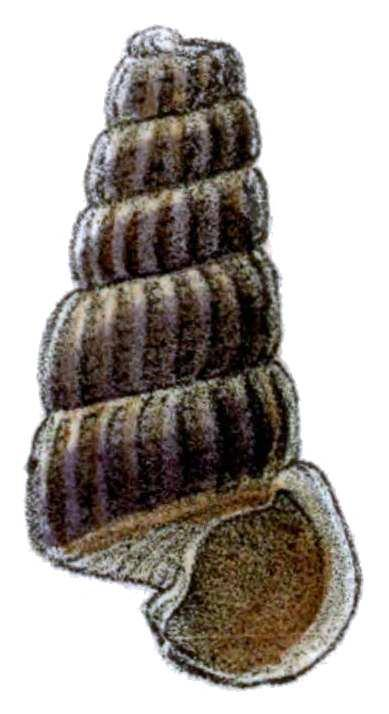
\includegraphics[scale=0.2]{shell.jpg}
                 \caption{Cerithidea Decollata.}
                 \end{center}
			\end{figure}
			
			The adults have a shell about 3 \textit{cm} long formed by 5 coils, usually with the broken tip, with about 20 ribs for each coil.\\
			These snails proliferate in coastal mangroves , particularly in the western part of Kenya, Tanzania, Mozambique , South Africa and Madagascar.\\
			The \textit{Cerithidea decollata} mainly feeds on algae and organic debris carried by the tide. That's why they live mainly in intertidal zones (coastal areas that depend on the tide), which has two high tides  and low tides every day.\\
			Every time the tide lowers, these snails descend to the ground to feed. Then, from one to two hours before the tide rises they begin to climb the trunk of the nearby trees, to stop from 20 to 60 \textit{cm} above the level of the incoming tide, waiting for it to rise and lower again.\\
			This behaviour allows them to avoid adverse physiological effects related to diving and to escape possible marine predators (like crabs). It is unclear, however, how these snails may be able to foresee the height of the incoming tide.\\
			In this study we will not dwell on how the \textit{Cerithidea decollata} may actually be able to predict the height of the tides, but only on which is the minimal neural network required to perform such prediction.\\
			So, for simplicity, we will assume that these snails are able to observe, at fixed intervals, the current level of the sea and, on the basis of these informations, to predict the tide level after a fixed number of hours.
		
		\subsection{Tide}
				
			Tides are caused mainly by the combination of two factors:
			\begin{itemize}
				\item the attraction of Sun and Moon over Earth; 
				\item the centrifugal force caused by the rotation of the Earth-Moon system around its centre of mass.
			\end{itemize}

			The height and frequency of the tide vary on the location and on the moment of the year. In general there are two high tides and two low tides every day. 
			For the studies we propose in this paper has been used a time dependent formula (expressed in hours, as shown below), which approximates the tide function:
			
			\[f(t) = A_a \cos \left(\frac{2 \pi t}{T_a}\right) + A_b \cos \left(\frac{2 \pi t}{T_b}\right) - D \sin \left(\frac{\pi t}{T_m} - \frac{\pi}{4}\right)\]
			
			In particular, we assigned the following values to the variables in the previous formula:
			\begin{itemize}
			\item $A_a=1.06$
			\item $A_b=0.65$
			\item $D=0.15$
			\item $T_a=12.42$
			\item $T_b=12$
			\item $T_m=12.21$
			\end{itemize}
			With this approximation the tide have a full period of about 28 days. 
			 
			\begin{figure}[h]
				\centering
				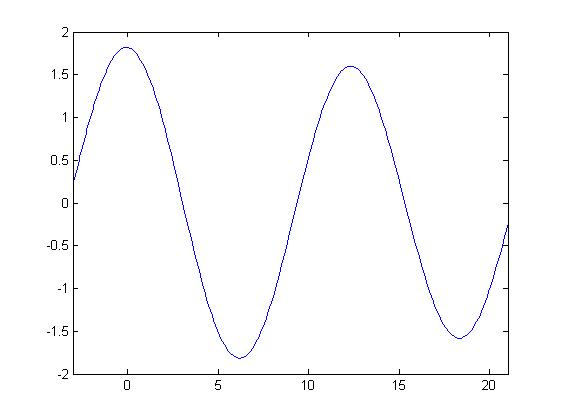
\includegraphics[scale=0.6]{tide_one_day.jpg}
				\caption{Tide function in a day.}
			\end{figure}

			\begin{figure}[h]
				\centering
				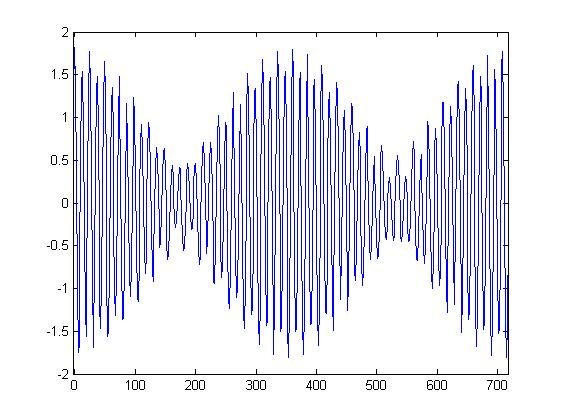
\includegraphics[scale=0.6]{tide_one_month.jpg}
				\caption{Tide function in a month.}
			\end{figure}
			
		\subsection{Neural Networks}
			To simulate the snail neural network and the subsequent study of the neural complexity required to perform such prediction, it was decided to start with a Widrow network. \\
			With this very simple type of neural network we obtained, as we will see in greater detail in the following two chapters, excellent results. So, regarding the simple prediction and the prediction with errors, it was not necessary to try more complex networks.\\
			However, for the study of more complex problems (like next tide peak prediction or new altitudes adaptation) a simple linear network was not sufficient and a Multilayer Perceptron (a more complex type of neural network) has been used.
			\subsubsection{Widrow Network}
				The Widrow-Hoff network is a class of adaptive filters called  ADALINE.\\
				The network is composed of a single output layer and uses a sum and a learning function. Each input \textit{x} of the network has an associated weight \textit{w}; the output corresponding to an input set is calculated simply with the weighted average:
				
				\[y = \sum_{j=1}^{n} x_j w_j\]
				
				The structure is very similar to that of the simple Perceptron and, more in general, to the McCulloch-Pitts neural model. However, it differs from it for the learning function: the Widrow-Hoff  learning algorithm (also called $\alpha$-LMS) updates, at each iteration, the weights based on the inputs weighted average.\\
				Without going into more technical details, the resulting learning algorithm is as follows:
				
				\[w_{k+1} = w_k + \alpha(t_k - y_k)\frac{x_k}{|x_k|^2}\]
				
				The network has been trained on a 20'000 inputs vector, for the simple prediction and with errors, and 10'000 inputs, for all subsequent predictions. Each one of these training inputs is formed by 5 different hours at a fixed distance from one another, randomly distributed over 28 days.
				
			\subsubsection{Multilayer Perceptron}
				The Multilayer Perceptron is the natural evolution of the standard Perceptron. It basically adds to the Perceptron one or more intermediate (or hidden) layers of neurons between the input layer and the output layer.\\
				The greatest advantage of the Multilayer Perceptron, compared to the standard one, is that it's able to solve nonlinear problems and therefore can be applied to those problems that the simple Perceptron just can't solve.
				
				\begin{figure}[h]
					\centering
					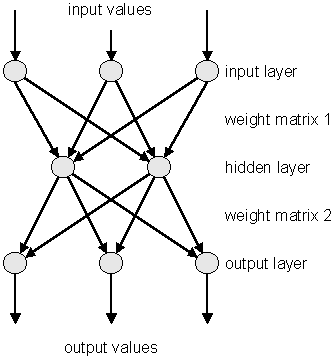
\includegraphics[scale=0.6]{multi.png}
					\caption{Multilayer Perceptron structure.}
				\end{figure}
				
				In the simulations performed in this article the transfer functions used are \textit{logsig}, i.e. the logistic function, for the hidden layer, and \textit{purelin}, i.e. the linear transfer function, for the output layer. The learning function used in this case is \textit{trainlm}, which corresponds to the Levenberg-Marquardt backpropagation rule.\\
				The network learning was carried out on 10'000 sets of hours, each consisting of 5 hours at a distance of 1 hour from each other.
	
	\section{Simple prediction}
		As already mentioned in the introduction, we take for granted that these snails are able to observe a fixed number of tide heights, within a fixed distance, and then predict the tide height after an arbitrary number of hours.\\
		With simple prediction we mean the simulation of the prediction of the future tide height by the \textit{Cerithidea decollata} in an error-free environment, i.e. a situation in which the snail is able to observe the heights of tide with absolute precision and to evaluate time intervals with the same accuracy. 
		\subsection{Simple prediction two hours away}
			To get as close as possible to the behaviour of the \textit{Cerithidea decollata} the first simulations have been those in which the snail observes 5 tide heights, each at a distance of half an hour from each other, and then perform the prediction of the tide height two hours later.\\
			From these simulations we have obtained excellent results: the standard deviation reached during the training on 28 days is around $10^{-5}$, which, considering that the tide function takes values between -2 and 2, and therefore the maximum possible absolute error is of the order of 4, means that averagely the snails predict the tide height (two hours later) with an error of about \textbf{0.0006\%}.\\
			In the plots obtained after these simulations the blue line indicates the exact tide function, the points circled in blue indicate the tide heights observed before the prediction and the cross and the red circle indicate, respectively, the foreseen tide height and the actual tide height two hours later.
	
      		\begin{figure}
		        \begin{center}
		        	\begin{subfigure}{0.4\linewidth}
						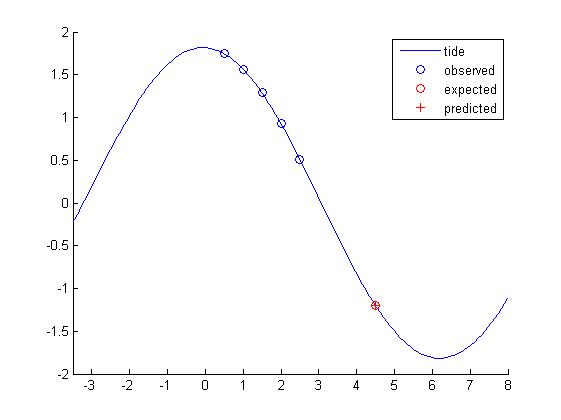
\includegraphics[scale=0.3]{simple_2h_1.jpg}
					\end{subfigure}\qquad
		        	\begin{subfigure}{0.4\linewidth}
						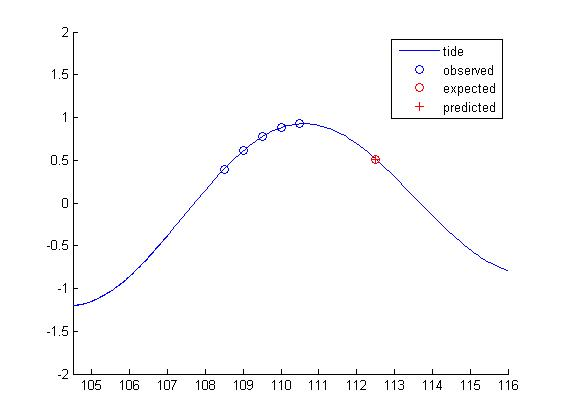
\includegraphics[scale=0.3]{simple_2h_2.jpg}
					\end{subfigure}\\
		        	\begin{subfigure}{0.4\linewidth}
						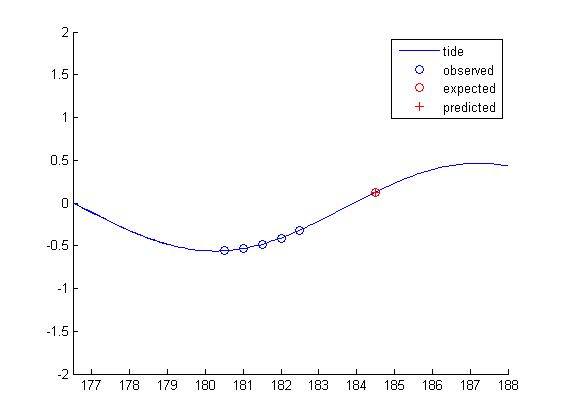
\includegraphics[scale=0.3]{simple_2h_3.jpg}
					\end{subfigure}\qquad
		        	\begin{subfigure}{0.4\linewidth}
						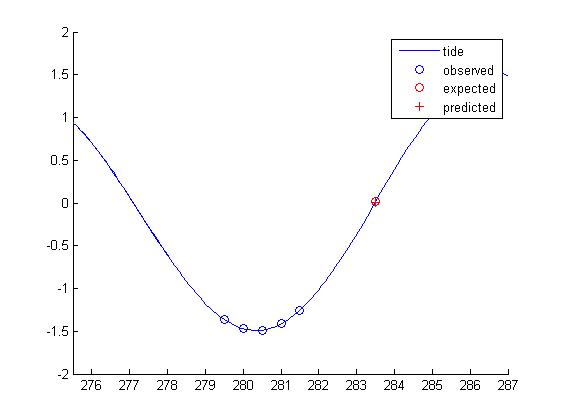
\includegraphics[scale=0.3]{simple_2h_4.jpg}
					\end{subfigure}
					\caption{Simulations of the simple prediction two hours away.}
		        \end{center}
			\end{figure}
			\FloatBarrier
	\section{Prediction with errors}
		We have seen in the previous section that the simple prediction (i.e.,  error-free), has given excellent results.\\
		We now study the tide height prediction by adding errors in the perception that the snails have about the environment and the situation.\\
		The errors introduced will therefore be of two types: errors in the evaluation of the tide height observed and errors on the estimation of the elapsed time between each observation and the next one.\\
		It is conceivable to think that these snails have not a perfect measurement system for the tide heights or the passage of time, therefore relying on an estimation, more or less accurate.\\
		In the simulations performed in this chapter we used tide height errors of maximum 0.6 (in absolute value, then between -0.6 and 0.6 ), which represents a maximum error of 15\% on the tide height observed, and a time interval error of about (maximum) 16\%. Regarding the tide height errors, it was decided to assign the same error in all 5 consecutive observations as it was assumed that, even if the snail won't be able to determine the tide height with absolute precision, it would be certainly easier for them to understand if the tide has raised or lowered by comparing the observations.
		\subsection{Prediction with errors two hours away}
			As in the previous chapter, we will try now to determine with which degree of error these snails are able to predict the tide two hours away after 5 observations half an hour away from each other.\\
			The standard deviation obtained with this type of simulations is of about 0.124, which corresponds to \textbf{3.1\%} on the tide height. This immediately tells us that the prediction with errors turns out to be more complex and more difficult to accomplish than the simple one.\\
			If we compare this result with that obtained in the simple predictions two hours away (average error of less than 0.0006\%) we see that the error is increased by a \textbf{factor of} about \textbf{5000}. Of course an average error of 3.1\% is still a widely acceptable result, but this makes us realize how small mistakes on sensory data can lead to a huge increase in complexity for the prediction of future tides, especially for the random nature that these errors have.
	
      		\begin{figure}
		        \begin{center}
		        	\begin{subfigure}{0.4\linewidth}
						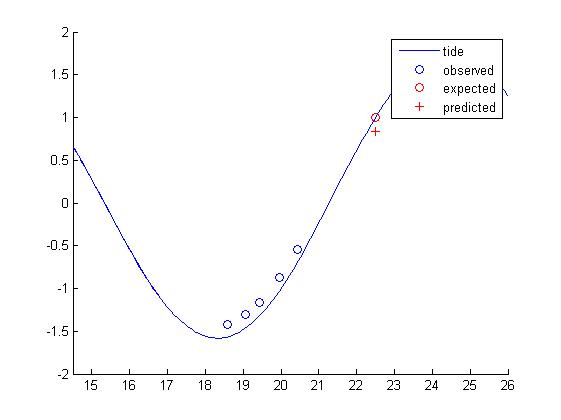
\includegraphics[scale=0.3]{error_2h_1.jpg}
					\end{subfigure}\qquad
		        	\begin{subfigure}{0.4\linewidth}
						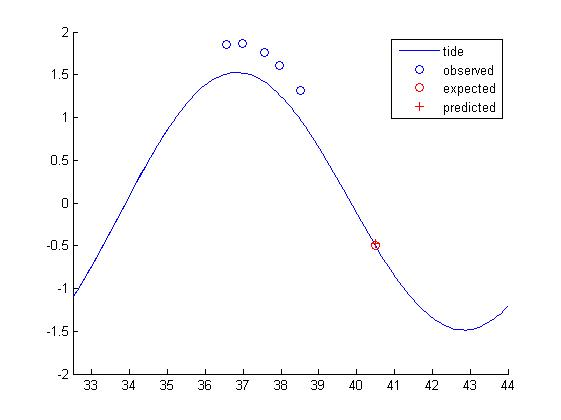
\includegraphics[scale=0.3]{error_2h_2.jpg}
					\end{subfigure}\\
		        	\begin{subfigure}{0.4\linewidth}
						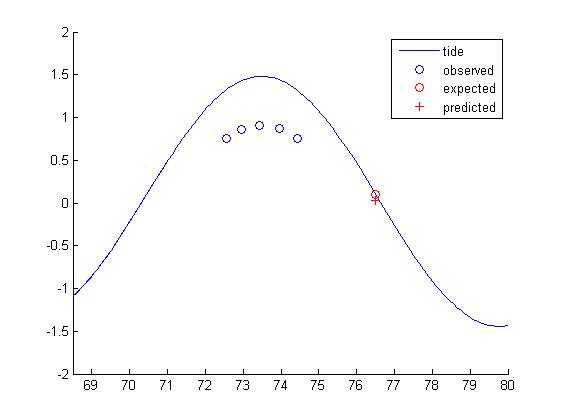
\includegraphics[scale=0.3]{error_2h_3.jpg}
					\end{subfigure}\qquad
		        	\begin{subfigure}{0.4\linewidth}
						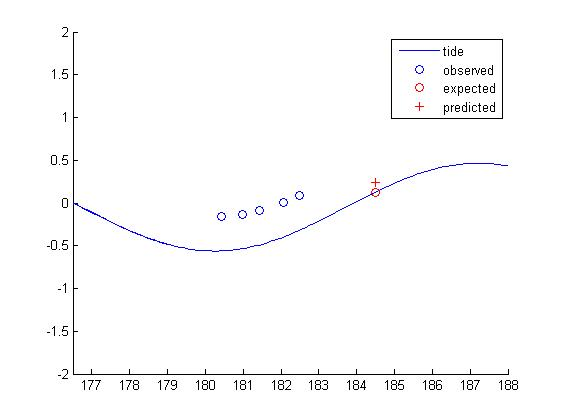
\includegraphics[scale=0.3]{error_2h_4.jpg}
					\end{subfigure}
					\caption{Simulations of the prediction with errors two hours away.}
		        \end{center}
			\end{figure}
			\FloatBarrier
	\section{Next tide peak prediction}
		In addition to the predictions after a fixed number of hours (last two chapters) another important experiment is that of the prediction of the next tide peak. As in the previous chapters, the snail observes 5 tide heights, this time 1 hour away from each other, and then predicts in how many hours will be the next high tide and the altitude of that peak.\\
		Regarding sensory errors to which the snail  may be subject it was decided to maintain the 15\% error on the water level perception and 16\% on the perception of the passage of time (corresponding to $\pm 10$ minutes, being in this case an hour the interval between two successive observations).\\
		In these scenario, the errors have to be calculated as the average of the two errors (i.e., temporal errors and altitude errors). So if we consider a maximum absolute error of 4 in the altitude axis and of 13 in the time axis (since there is at least one peak every 12 hours), we have a maximum absolute error of 8.5.\\
		\\
		As expected, a simple Widrow Network was insufficient for these kind of predictions. In fact, running these simulations we registered an average error (on both time and altitude) of 39.5\%. This tells us that for more realistic simulations, a more complex neural network is needed.
		\subsection{Prediction with Multilayer Perceptron}
			The following attempt has been with a feed-forward network, in particular a Multilayer Perceptron.\\
			We immediately noticed that this type of network responds much better to the prediction of the next tide peak than the simple Widrow Network, so we tried to find the minimum number of neurons in the hidden layer so that the total average error could fall below an acceptable value, which we thought should be fixed at \textbf{12\%}.\\
			The result was that \textbf{6 neurons} represent the minimum to have an error less than or equal to 1.02, which corresponds precisely to 12\% over 8.5. Obviously, the more neurons we introduce, the lower the error will be, but the growth is very slow compared to the number of neurons needed, so a 12\% error with 6 neurons seems to be a good compromise.
	
      		\begin{figure}
		        \begin{center}
		        	\begin{subfigure}{0.4\linewidth}
						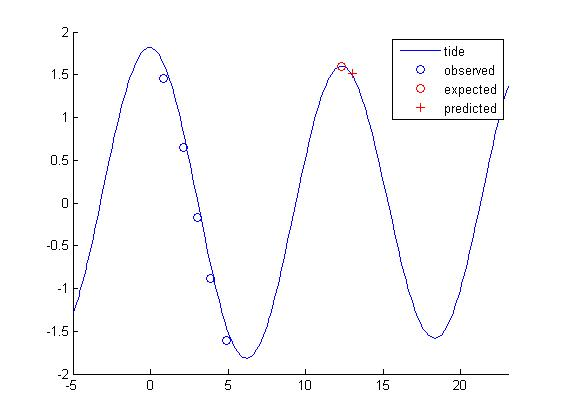
\includegraphics[scale=0.3]{edge_ff_1.jpg}
					\end{subfigure}\qquad
		        	\begin{subfigure}{0.4\linewidth}
						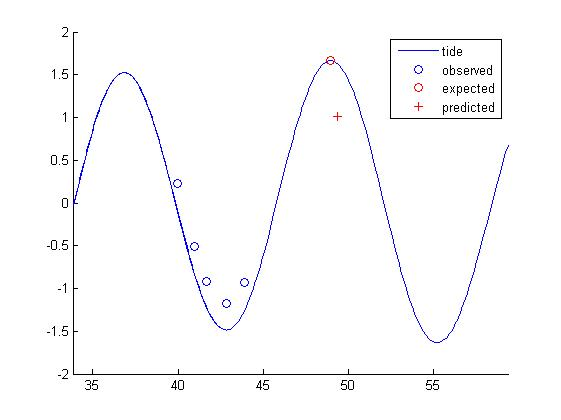
\includegraphics[scale=0.3]{edge_ff_2.jpg}
					\end{subfigure}\\
		        	\begin{subfigure}{0.4\linewidth}
						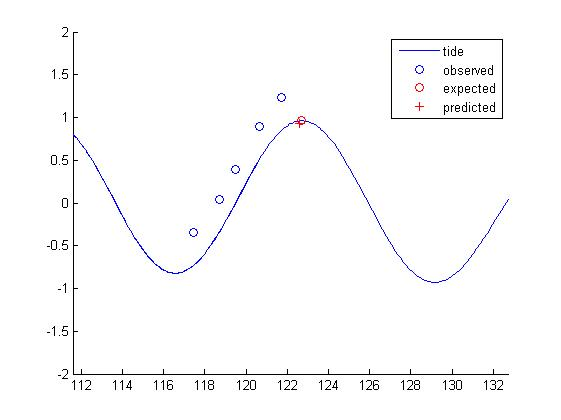
\includegraphics[scale=0.3]{edge_ff_3.jpg}
					\end{subfigure}\qquad
		        	\begin{subfigure}{0.4\linewidth}
						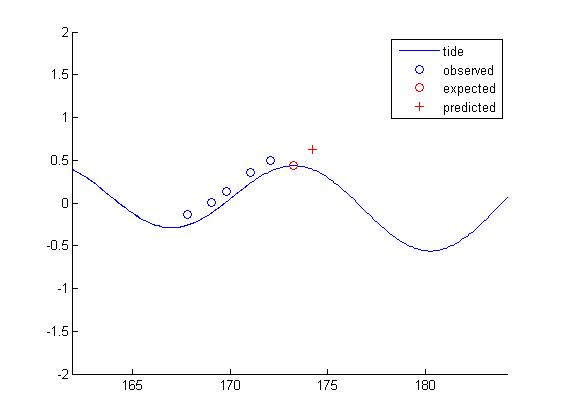
\includegraphics[scale=0.3]{edge_ff_4.jpg}
					\end{subfigure}
					\caption{Simulations of the next tide peak prediction with Multilayer Perceptron.}
		        \end{center}
			\end{figure}
			\FloatBarrier
	\section{Peak observation and prediction}
		In this chapter we will examine the problem in which the snail observe the starting, peak and ending moments of the high tide and the height reached in the peak time of 3 consecutive high tides above the ground level, and then make a prediction on the starting, peak and ending  time of the next high tide, as well as the height reached by the tide during the peak.\\
		We then set the ground level to 0.5, where 0 is the sea level in the absence of tides and 2 is the highest possible peak of the tide (during the entire tide cycle). The errors introduced on the input data correspond to 10\% on tide level perception and a time error, of maximum 5 minutes.
		The network (a Multilayer Perceptron) training is done using 500 random pattern of example input data, with the corresponding output target.\\
		The result is that the minimum number of neurons in the hidden layer needed to achieve an average error of about \textbf{0.1\%}, is \textbf{17 neurons}. To obtain, however, a mean error of less than \textbf{1\%} only \textbf{4 neurons} are needed, while for errors of less than \textbf{5\%}, \textbf{2 neurons} appear to be sufficient.\\
		As one might expect from such a prediction, the network simulates much better when we  have the 3 high tides observed and the high tide to be predicted consecutive (i.e., 4 successive tides that exceed the level of the ground). In fact for this type of prediction works very well even the most simple networks, even with 10 neurons. However, especially during periods of neap tide, or when the moon is in quadrature, high tides may not be able to exceed the level of the ground and we may also get to see whole days without a single tide or high tide per day (instead of two, as during the spring tide). In these cases it is required just a minimally more complex neural network, since determining when a new high tide will raise above the ground level again involves much complex calculations.
		
		\begin{figure}
			\begin{center}
				\begin{subfigure}{0.4\linewidth}
					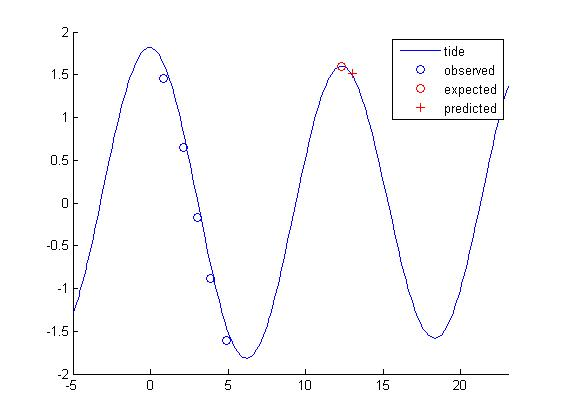
\includegraphics[scale=0.3]{edge_ff_1.jpg}
				\end{subfigure}\qquad
				\begin{subfigure}{0.4\linewidth}
					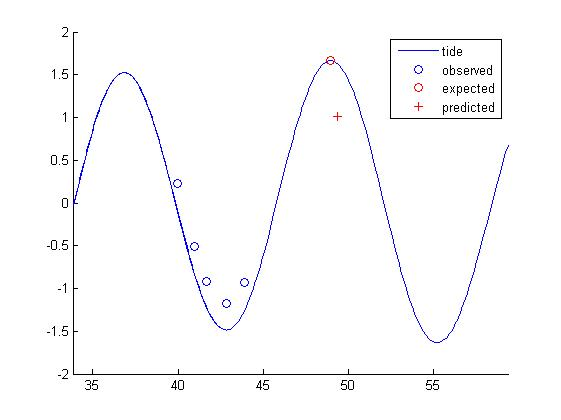
\includegraphics[scale=0.3]{edge_ff_2.jpg}
				\end{subfigure}\\
				\begin{subfigure}{0.4\linewidth}
					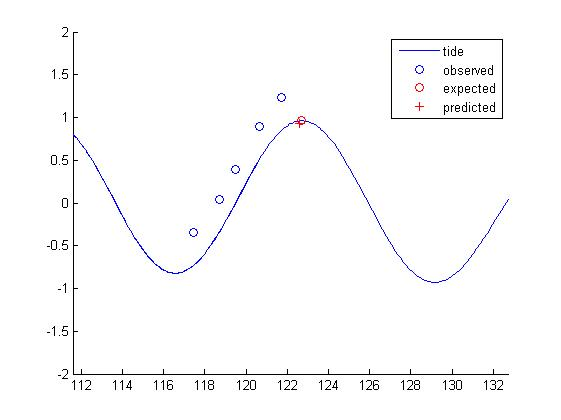
\includegraphics[scale=0.3]{edge_ff_3.jpg}
				\end{subfigure}\qquad
				\begin{subfigure}{0.4\linewidth}
					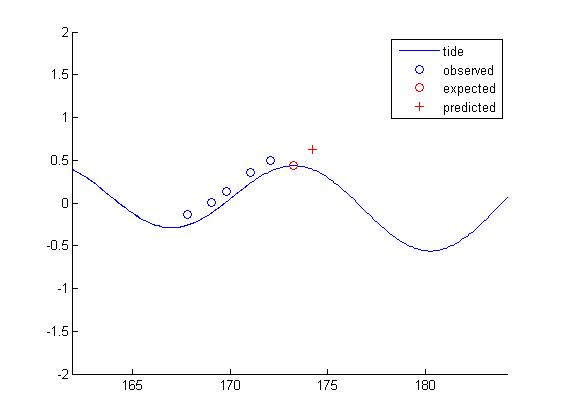
\includegraphics[scale=0.3]{edge_ff_4.jpg}
				\end{subfigure}
				\caption{Simulations of the peak observation and prediction.}
			\end{center}
		\end{figure}
		\FloatBarrier
	\section{Adaptation to new altitudes}
		After trying to estimate, in the last chapters, the minimum neural network capable of performing various types of tide forecasting, we will enter now more in detail into the problem, trying to build a more accurate neural network model of the \textit{Cerithidea decollata}.\\
		In particular, in this chapter we will attempt to reproduce an experiment conducted by Prof. Vannini, in which the specimens of \textit{Cherithidea decollata}, living at a given altitude, are moved to a new altitude (in this case, lowest than the native one), to study how the snails adapt to the new the scenario. Of course, moving the snails from a higher point to a lower one is much more interesting than the other way around, since these snails have very few informations about the tide (they can spend many days without even having a tide) and have to do a lot of calculations to adapt to the more "aggressive" tide of the lower altitude.\\
		First of all, we made some changes to the model described in the previous chapters. The observations consist now only in observing the arrival time of the tide (i.e., when it exceeds the level of the ground) and arrival time and height of the tide peak. The observation of the tide ebb has been removed, as it was redundant knowing the first two informations (times of arrival and peak of the tide). It was also introduced a memory for these snails, which lasts about 28 days (i.e. a full tidal cycle), and the ability to use or not a lunar clock to help the snails in the forecasting process.\\
		It was then used a feed-forward neural network (as seen in the previous chapters, a Multilayer Perceptron) with \textbf{8 neurons} in the hidden layer, initially trained on a set of inputs at the native altitude, fixed at 1.5 (with 2 as maximum possible tide peak, 0 as sea level and -2 as maximum possible tide ebb). Thus, the snails are "moved" to the new altitude, fixed at 0.5, and are then trained with the new informations, dividing the training into days.\\
		Every day, 4 tide observations are made, during which the snails will modify its neural network until it matches with both the newly acquired informations and the old informations they still have in memory. Then we update the snail memory, removing the 4 older observations and adding the 4 observations just made. Finally, we calculate the error that the snail would commit trying to foresee the tide in the current day and for the next 27 days. This process is repeated for as long as it takes until the error in foreseeing the tide arrival for the current day and the next 27 days (i.e., for an entire tidal cycle) results to be less than a fixed value, in this case \textbf{5\%}.\\
		Performing then a series of tests with the parameters listed above we have that the snails can adapt to the new altitude in about (averagely) \textbf{9 days} of training. It is not therefore necessary that they observe the full tidal cycle at the new altitude to be able to predict the tide with an average error of less than 5\%.\\
		It was also introduced a lunar clock, in this model, to study how it affects the predictions when the snails have this additional information. The results were rather disappointing: if we use just the moon clock, the snails can not adapt to the new altitude within the predetermined error; if used in conjunction with the direct observation of the tide, there have been no significant improvements: in most cases there are differences in a single day, or even none, as regards the training.\\
		A noteworthy observation concerns the fact that, by increasing the number of neurons of the neural network, the days required for matching increases. This is due to the fact that a greater number of neurons implies a greater complexity of the neural network and consequently a greater number of days necessary for the adaptation to the new altitude. This result points out, once again, that the neural network required for this type of forecast must be extremely simple.
		
		
		\begin{figure}
			\begin{center}
				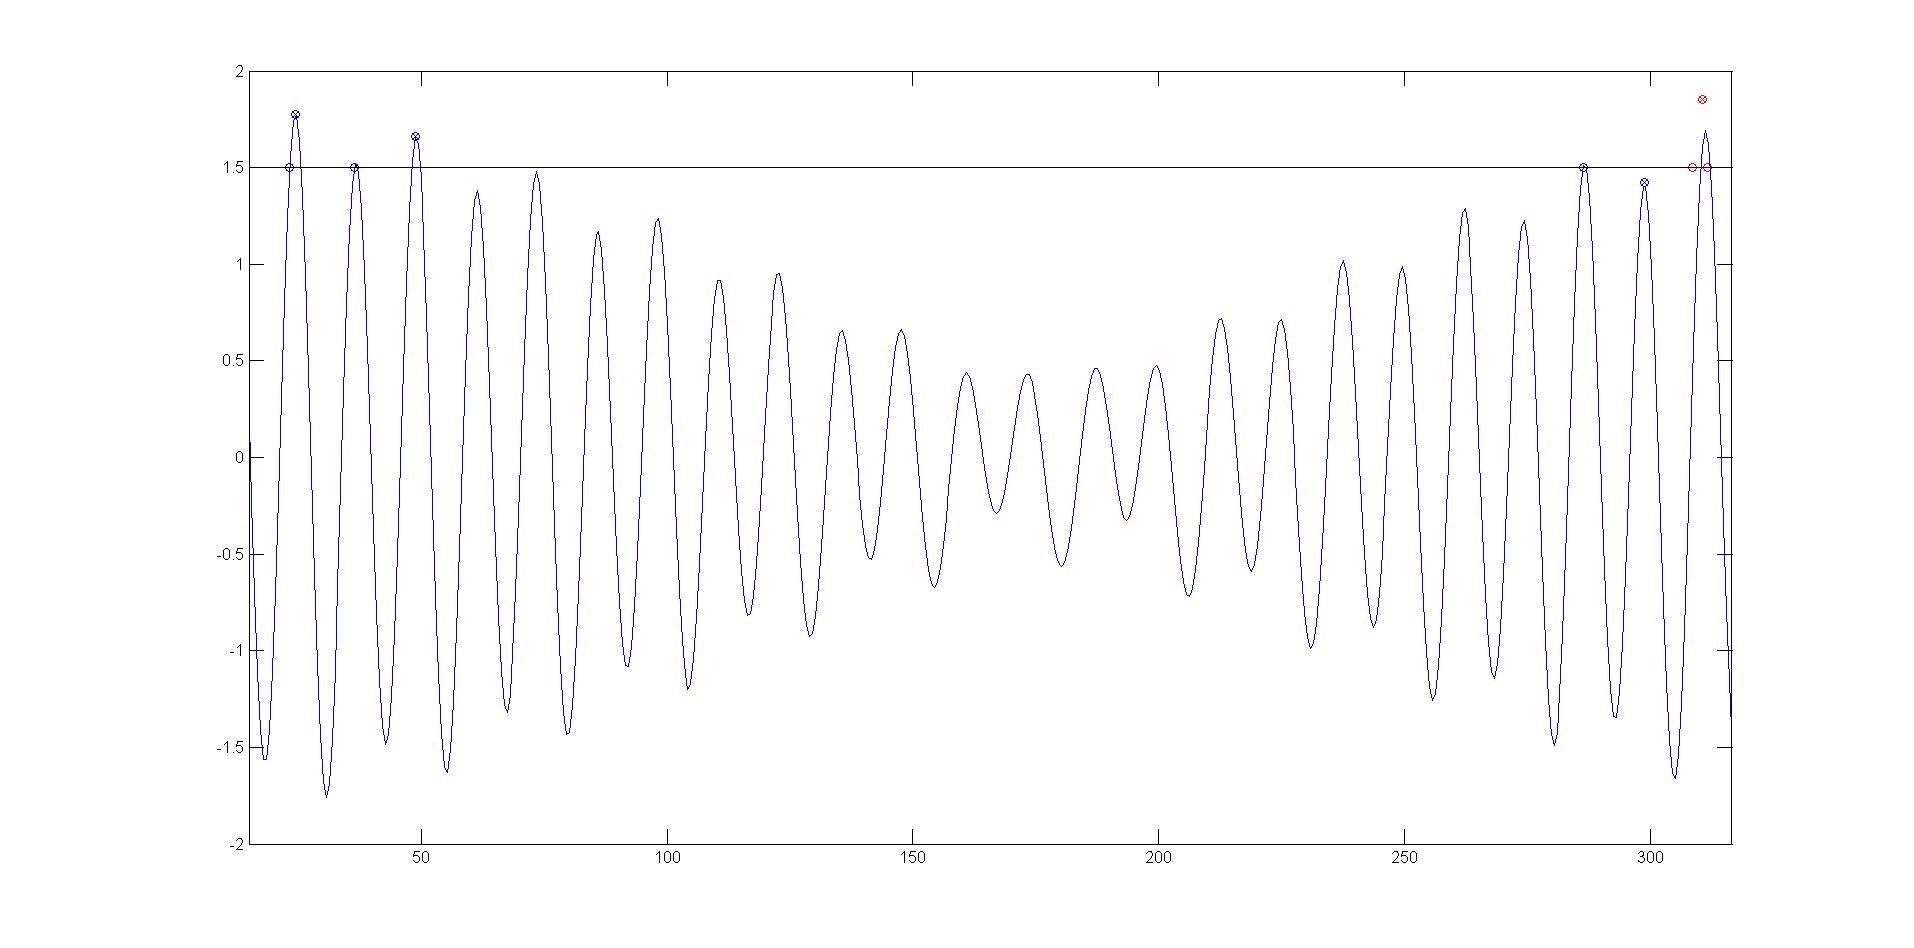
\includegraphics[scale=0.2]{adapt1_a.jpg}
				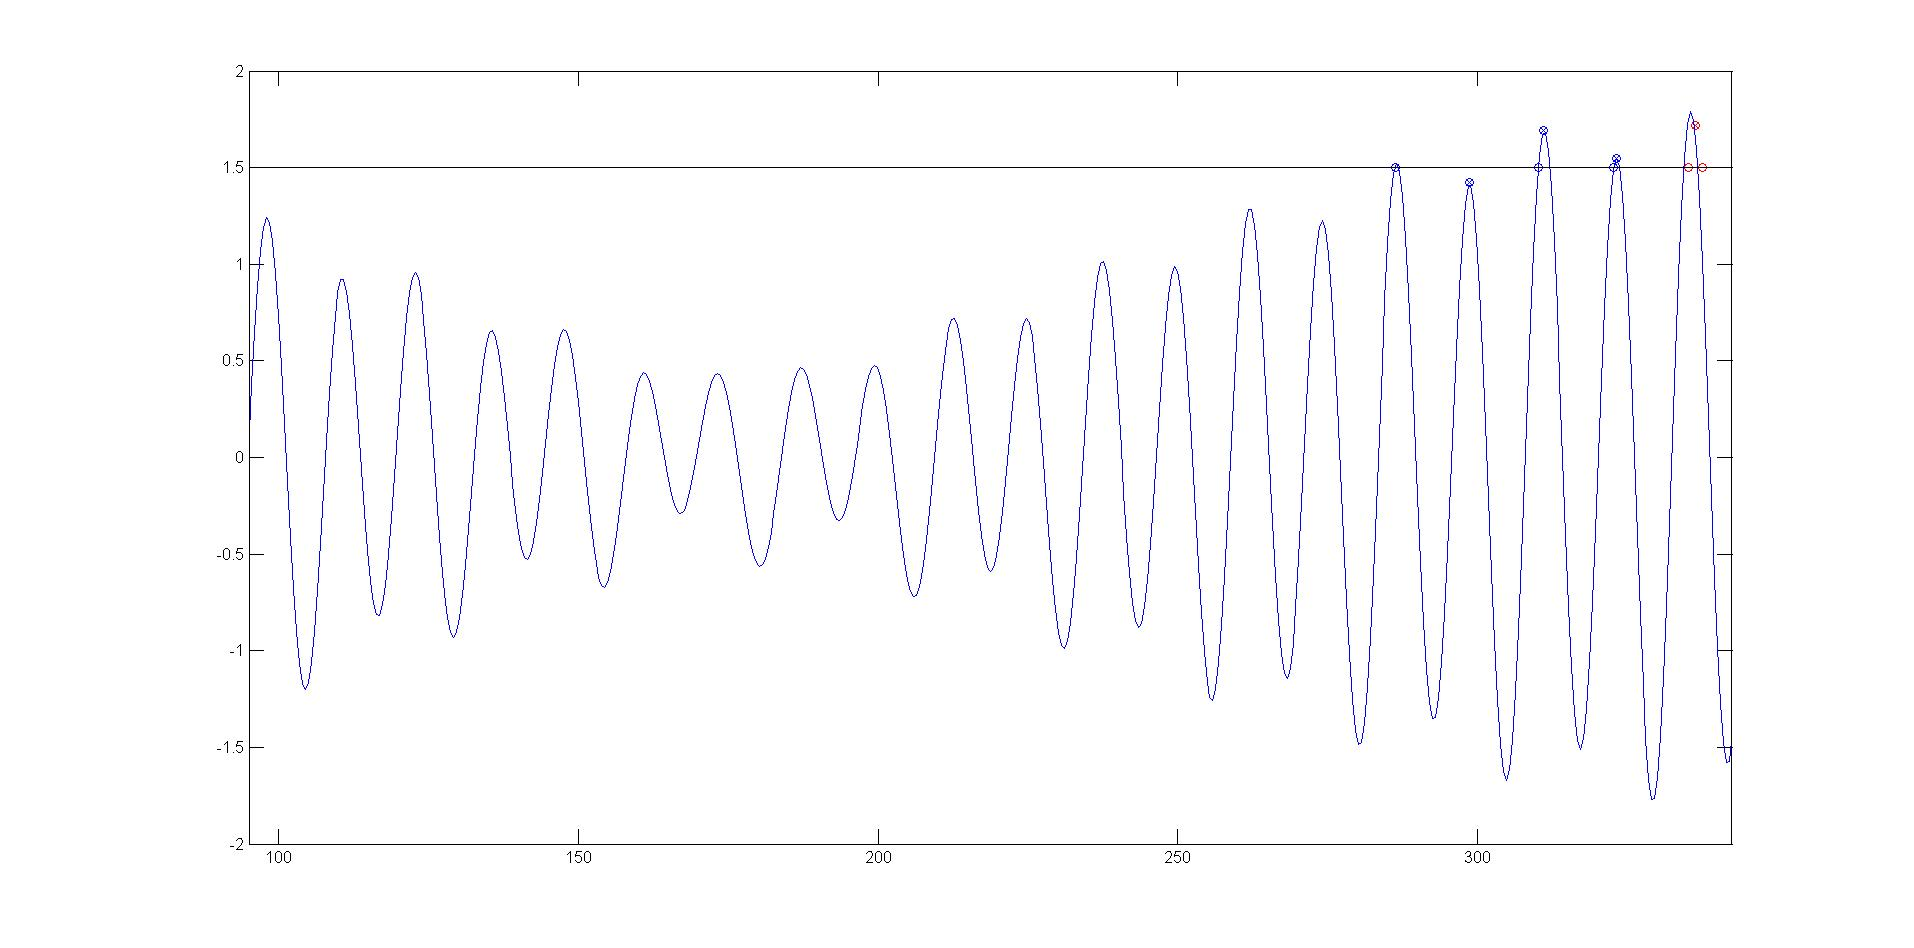
\includegraphics[scale=0.2]{adapt1_b.jpg}
				\caption{Simulations of the adaptation to new altitudes (before being moved).}
			\end{center}
		\end{figure}
		
		\begin{figure}
			\begin{center}
				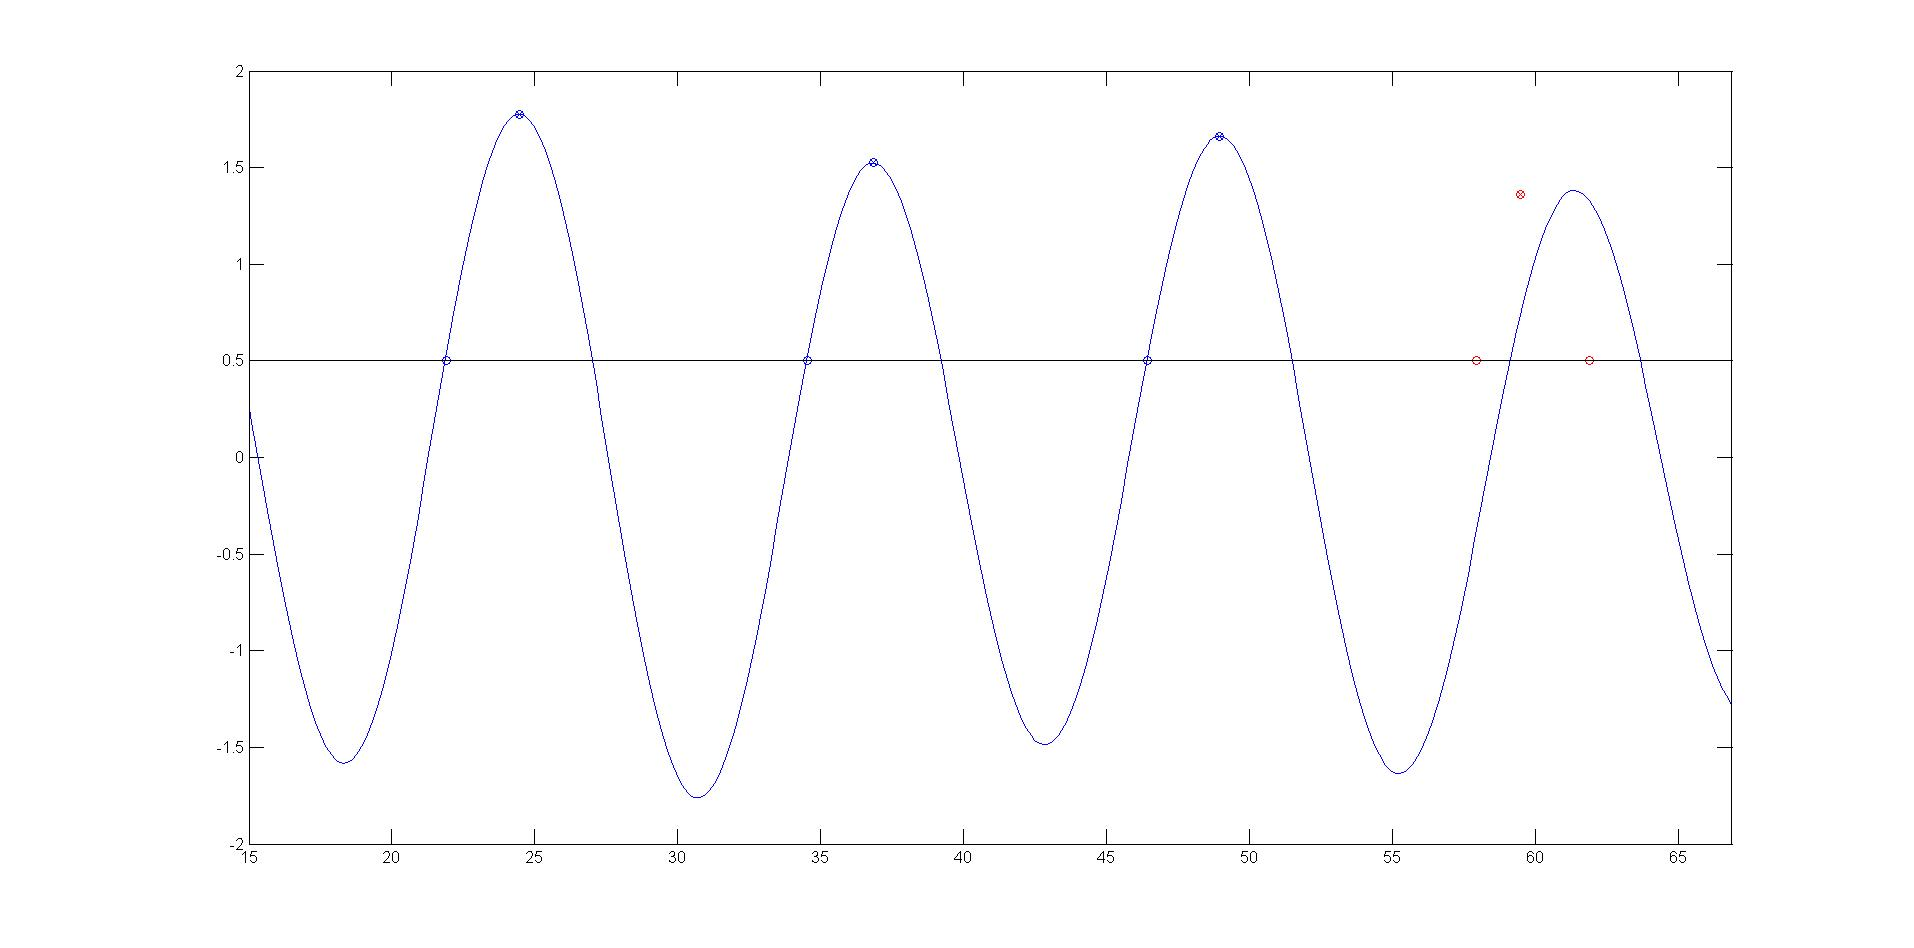
\includegraphics[scale=0.2]{adapt2_a.jpg}
				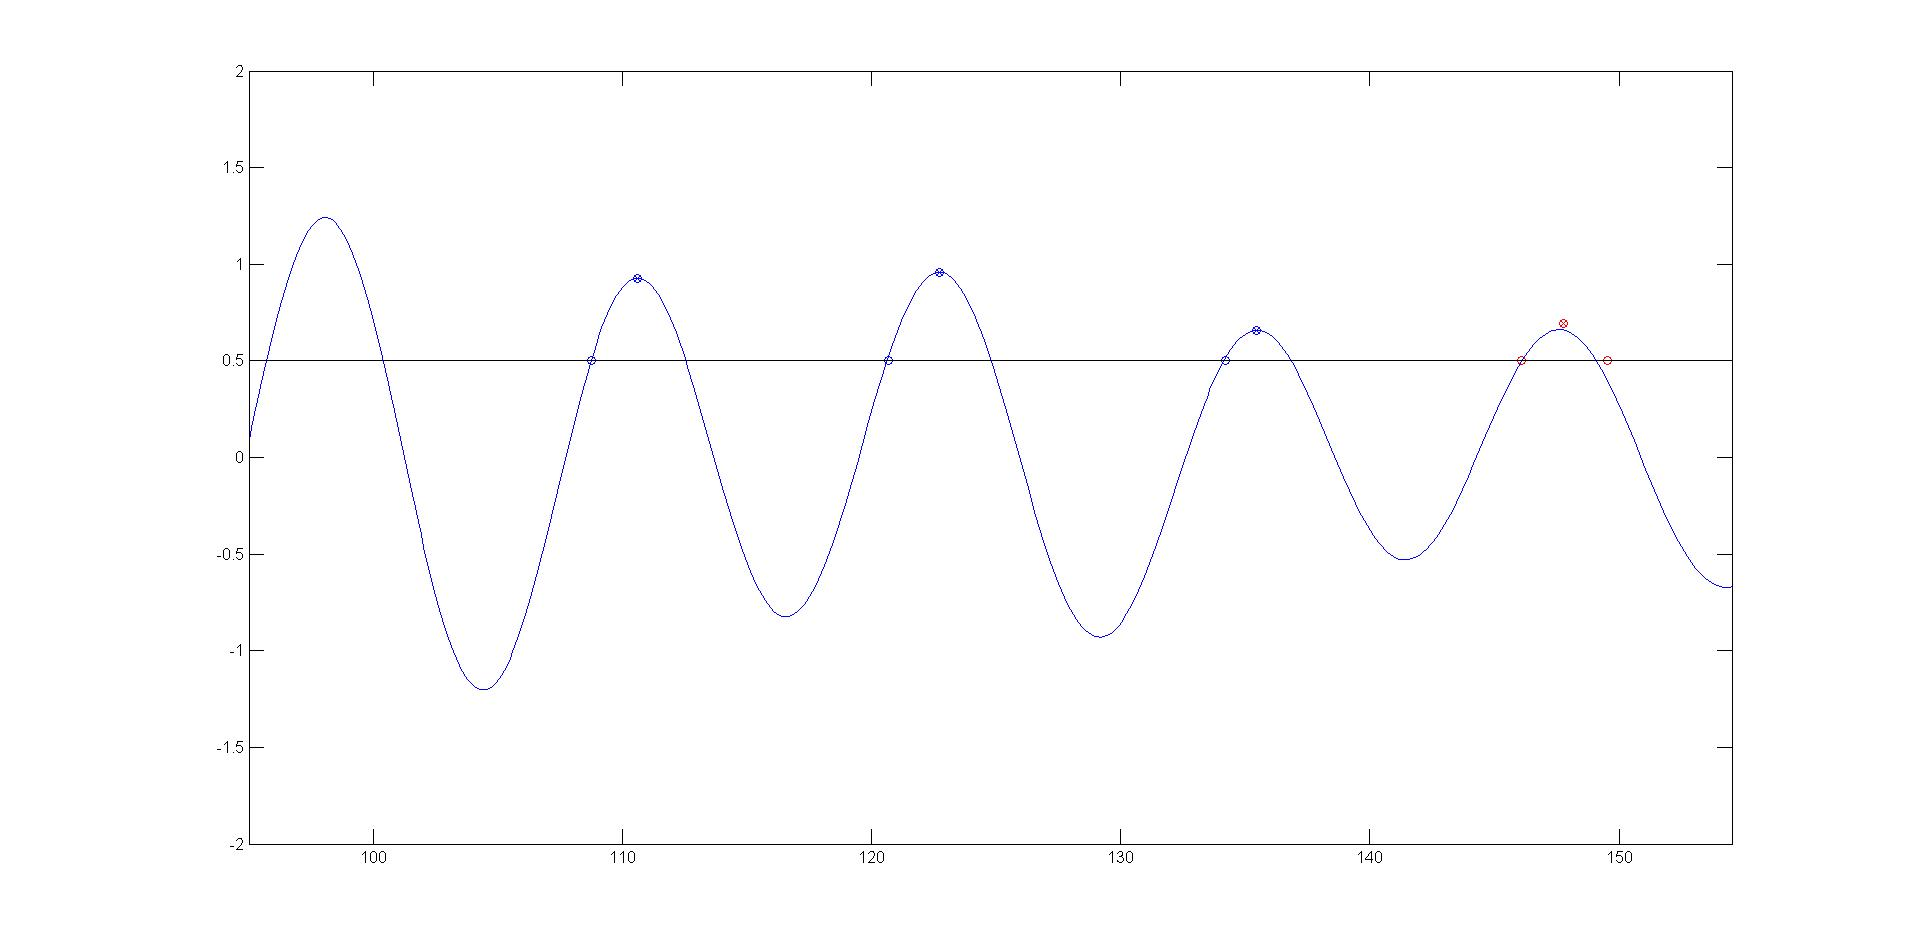
\includegraphics[scale=0.2]{adapt2_b.jpg}
				\caption{Simulations of the adaptation to new altitudes (after being moved).}
			\end{center}
		\end{figure}
	\FloatBarrier
	
	\section{Acknowledgments}
	
		Many thanks are due to Dr Renison Ruwa (KMFRI, Mombasa)  Dr. Mohamed Omar Said (KWS,  Mombasa) for their support and 
		encouragement in Kenya.  Many thanks to G. Landi for suggesting the neural network approach to our behavioural study.
	
	\begin{thebibliography}{99}
	
		\bibitem{chelazzi}Chelazzi, G., Focardi, S. and Deneuborg, J. L. 1983. A comparative study on the movement patterns of two sympatric tropical chitons (Mollusca: Polyplacophora). Marine Biology, 74: 115-125.
		
		\bibitem{cockcroft}Cockcroft, V. G. and Forbes, A. T. 1981. Tidal activity rhythms in the mangrove snail Cerithidea decollata (Linn.) (Gastropoda: Prosobranchia: Cerithiidae). South African Journal of Zoology, 16: 5-9.
		
		\bibitem{harumi}Harumi, O., Eiko, M. and Kiyonori, T. 2002. Tree climbing behavior of the snail Cerithidea rhizophorarum (Gastropoda: Potamididae). Venus, 61: 215-232.
		
		\bibitem{hodgson}Hodgson A. N and Dickens J., 2012. Activity of the mangrove snail Cerithidea decollata (Gastropoda: Potamididae) in a warm temperate South African estuary. Estuarine Coastal Shelf Sciences., 109: 98-196.
		
		\bibitem{macnae}Macnae, W. 1963. Mangrove swamps in South Africa. Journal of Ecology, 51: 1:25.
		
		\bibitem{mcguinness}McGuinness, K. A. 1994. The climbing behaviour of Cerithidea anticipata (Mollusca: Gastropoda) : 
		the role of physical versus biological factors. Australian Journal of Ecology, 19: 283-289.
		
		\bibitem{vannini}Vannini M. and Chelazzi, G. 1978. Field observations on the rhythmic behaviour of Nerita textilis 
		(Gastropoda: Prosobranchia). Marine Biology, 45: 113-121.
		
		\bibitem{vannini2}Vannini M., Rorandelli R.,  L�hteenoja O., Mrabu E. and Fratini S., 2006. Tree-climbing behaviour of Cerithidea decollata (L.), a Western Indian Ocean mangrove gastropod (Mollusca, Potamididae). Journal of marine biological Association, UK, 86: 1429-1436
		
		\bibitem{vannini3}Vannini M., Mrabu E., Cannicci S., Rorandelli R. and Fratini S., 2008a. Rhythmic vertical migration of the gastropod Cerithidea decollata in a Kenyan mangrove forest. Marine Biology, 153: 1047-1053
		
		\bibitem{vannini4}Vannini M., Lori E., Coffa C., Fratini S., 2008b. Cerithidea decollata, a snail that can foresee the future? Animal Behaviour, 76: 983-992
		
		\bibitem{vannini5}Vannini, M., Coffa, C., Lori, E., Fratini, S., 2008c. Vertical migrations of the mangrove snail Cerithidea decollata (L.) (Potamididae) through a synodic month. Estuarine Coastal Shelf Sciences, 78(4):644-648
	
	\end{thebibliography}

\end{document}
